\documentclass[9pt,border=10pt]{standalone}

\usepackage{tikz}
\usetikzlibrary{arrows,shapes,positioning,shadows,trees}

\renewcommand\familydefault{\sfdefault}

\begin{document}
\begin{tikzpicture}



\foreach \c [count=\i from 0] in {{Stretching},{Shrinking},{Finish Forming},{Flattening},{Doming},{Planishing},{Straightnening},{Edging}} 
    \pgfmathsetmacro\y{\i * 3.5} % Spacing
    \node at (\y,5) (Node\c) {};
    
    
\node[] at (NodeStretching) () {
\includegraphics[height=2.2cm]{Images/Stretching.png}};
\node[] at (NodeShrinking) () {
\includegraphics[height=2.2cm]{Images/Shrinking.png}};
\node[] at (NodeFinish Forming) () {
\includegraphics[height=2.2cm]{Images/Finish Forming.png}};
\node[] at (NodeFlattening) () {
\includegraphics[height=2.2cm]{Images/Flattening.png}};
\node[] at (NodeDoming) () {
\includegraphics[height=2.2cm]{Images/Doming.png}};
\node[] at (NodePlanishing) () {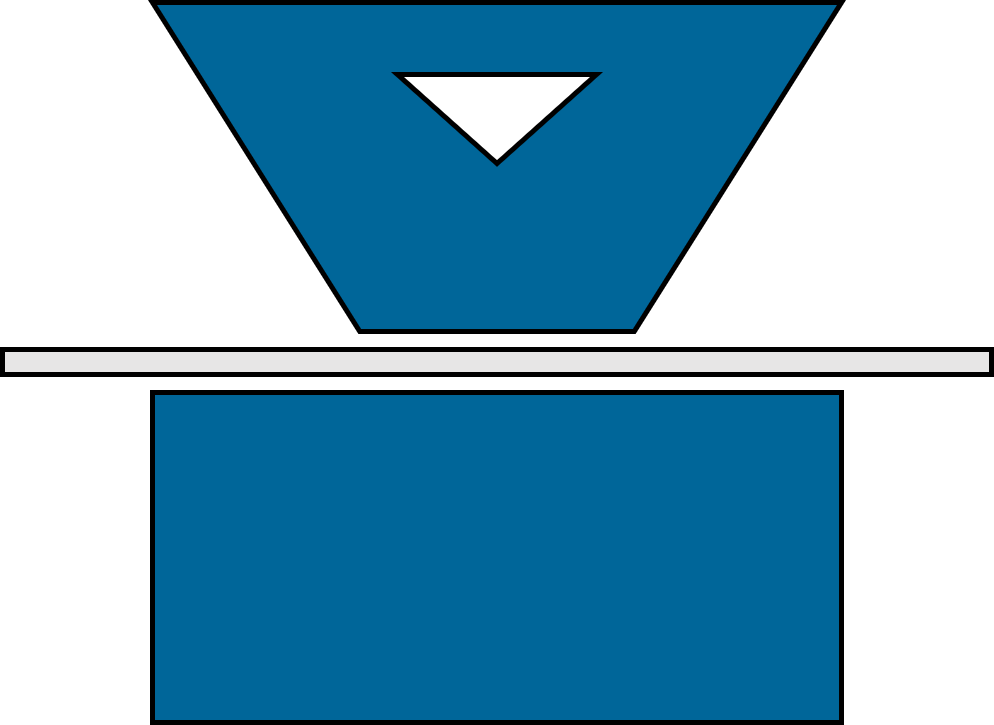
\includegraphics[height=2.2cm]{Images/Planishing.png}};
\node[] at (NodeStraightnening) () {
\includegraphics[height=2.2cm]{Images/Straightening.png}};
\node[] at (NodeEdging) () {
\includegraphics[height=2.2cm]{Images/Edging.png}};

\node[yshift=-1.7cm] at (NodeStretching) {(a)};
\node[yshift=-1.7cm] at (NodeShrinking) {(b)};
\node[yshift=-1.7cm] at (NodeFinish Forming) {(c)};
\node[yshift=-1.7cm] at (NodeFlattening) {(d)};
\node[yshift=-1.7cm] at (NodeDoming) {(e)};
\node[yshift=-1.7cm] at (NodePlanishing) {(f)};
\node[yshift=-1.7cm] at (NodeStraightnening) {(g)};
\node[yshift=-1.7cm] at (NodeEdging) {(h)};

\node[yshift=1.7cm] at (NodeStretching) {Stretching};
\node[yshift=1.7cm] at (NodeShrinking) {Shrinking};
\node[yshift=1.7cm] at (NodeFinish Forming) {Finish Forming};
\node[yshift=1.7cm] at (NodeFlattening) {Flattening};
\node[yshift=1.7cm] at (NodeDoming) {Doming};
\node[yshift=1.7cm] at (NodePlanishing) {Planishing};
\node[yshift=1.7cm] at (NodeStraightnening) {Straightnening};
\node[yshift=1.7cm] at (NodeEdging) {Edging};


%\node[] at (2,2) (StretchNode) {
\includegraphics[height=2.2cm]{Images/Stretching.png}};
%\node[yshift=-1.7cm,text width=5cm,align=center] at (StretchNode) {(a) \\Stretching};





\end{tikzpicture}
\end{document}